\section{Modellierung der Burg}

\subsection{Grundaufbau der Burg}

Als die Vorüberlegungen abgeschlossen waren, musste möglichst schnell ein grundlegendes Modell der Burg geschaffen werden. Dieses Modell sollte alle überlegten Maße einhalten und somit als Erstfassung dienen, um in eine Unity Szene eingefügt werden zu können.

\begin{figure}[h]
	\centering
	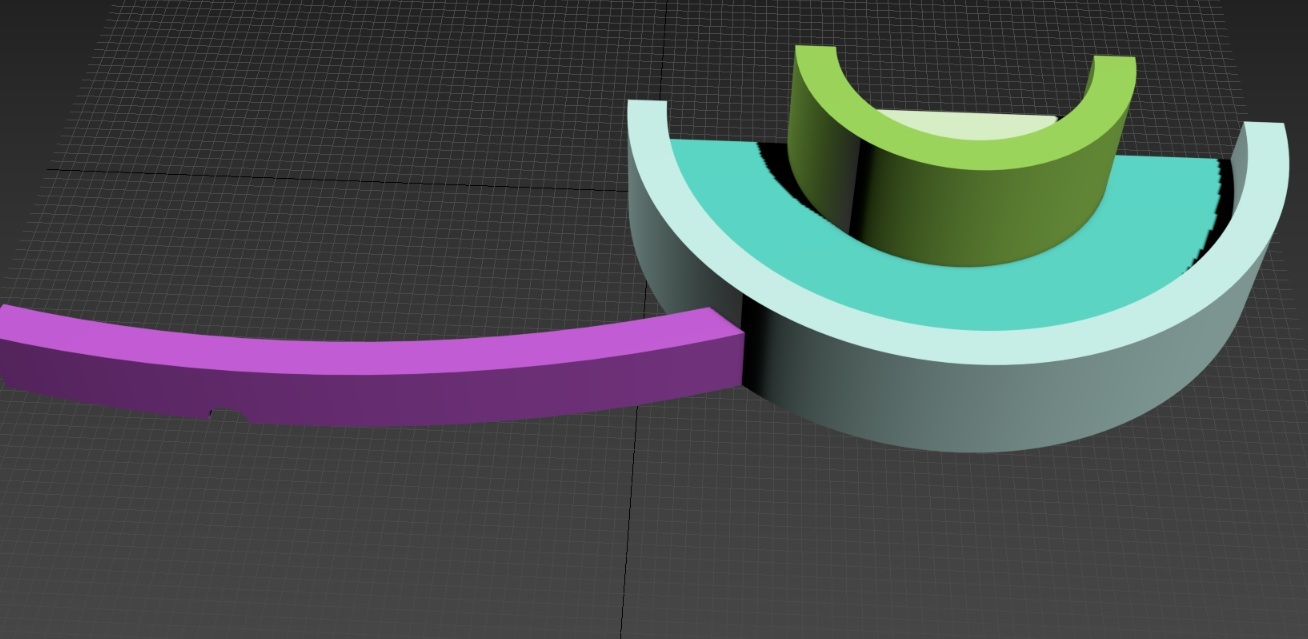
\includegraphics[width=0.95 \linewidth]{Abbildungen/3dsMax/Grundmodell}
	\caption{Grundaufbau der Burg}
	\label{fig:Grundaufbau}
\end{figure}

\begin{wrapfigure}{r}{0.5\textwidth}
	\begin{center}
		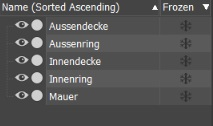
\includegraphics[width=0.45\textwidth]{Abbildungen/3dsMax/Grundhierachie}
	\end{center}
	\caption{Grundobjekte}
	\label{fig:Grundobjekte}
\end{wrapfigure}

Wie in den Abbildungen \ref{fig:Grundaufbau} und \ref{fig:Grundobjekte} zu sehen, besteht die Burg aus 5 Grundobjekten. Die Mauern wurden durch Röhren und die Decken durch Zylinder realisiert. Diese Objekte wurden anschließend in bearbeitbare Polys umgewandelt und zugeschnitten. Zum verschließen der daraus resultierenden offenen Enden wurde das Werkzeug \textit{Bridge} verwendet. Um später einen Fluss durch die lange Mauer fließen zu lassen, wurde unter Zuhilfenahme eines Zylinders und der boolschen Operation Subtrahieren eine halbrunde Öffnung hinzugefügt.

\newpage
\subsection{Modellierung des Haupttors}

\begin{figure}[h]
	\centering
	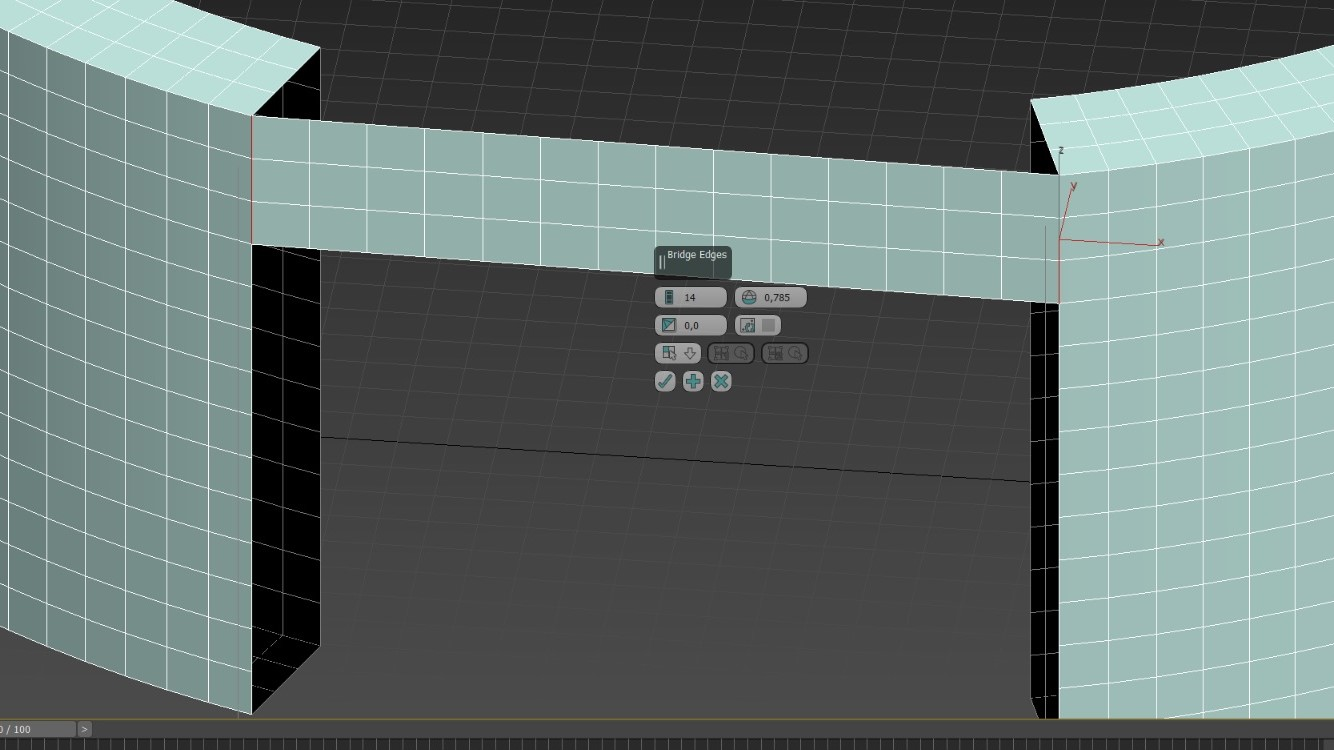
\includegraphics[width=0.95 \linewidth]{Abbildungen/3dsMax/Haupttor}
	\caption{Vorarbeit Haupttor}
	\label{fig:Haupttor}
\end{figure}

\begin{wrapfigure}{r}{0.5\textwidth}
	\begin{center}
		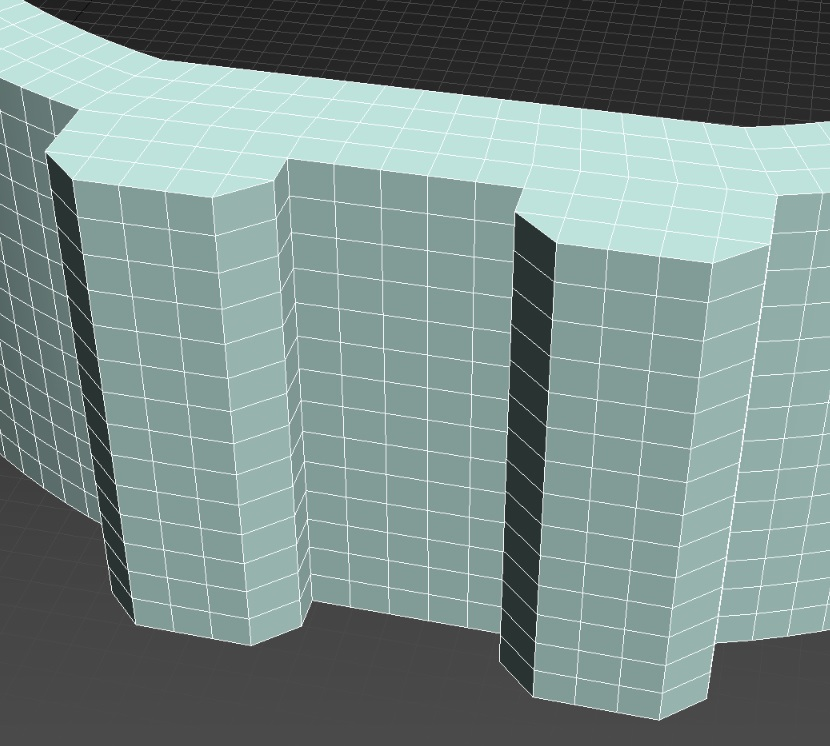
\includegraphics[width=0.45\textwidth]{Abbildungen/3dsMax/Haupttor2}
	\end{center}
	\caption{Haupttor}
	\label{fig:Haupttor2}
\end{wrapfigure}



Der nächste Schritt umfasste die Modellierung des Haupttores. Um eine gerade Arbeitsfläche zu erhalten, wurde der Mittelteil des Außenrings herausgeschnitten. Die nun freilegenden Kanten wurden, wie in Abb. \ref{fig:Haupttor} zu sehen mit dem \textit{Bridge} Werkzeug verbunden. Die Türme des Tores wurden anschließend mit dem \textit{Extrude} Werkzeug herausgearbeitet. Wie in Abb. \ref{fig:Haupttor2} zu sehen sind die frontalen Ecken der Türme "abgeschnitten". Um dies zu erreichen gibt es in 3dsMax verschiedene Möglichkeiten. In diesem Fall wurde das Kantenwerkzeug \textit{Chamfer} benutzt. Dies erlaubt es Ecken durch automatisches hinzufügen neuer Kanten abzurunden. Um das gewünschte Ziel zu erreichen wurde die Kantenanzahl verdoppelt.

\newpage
\subsection{Treppenbau}

\begin{figure}[h]
	\centering
	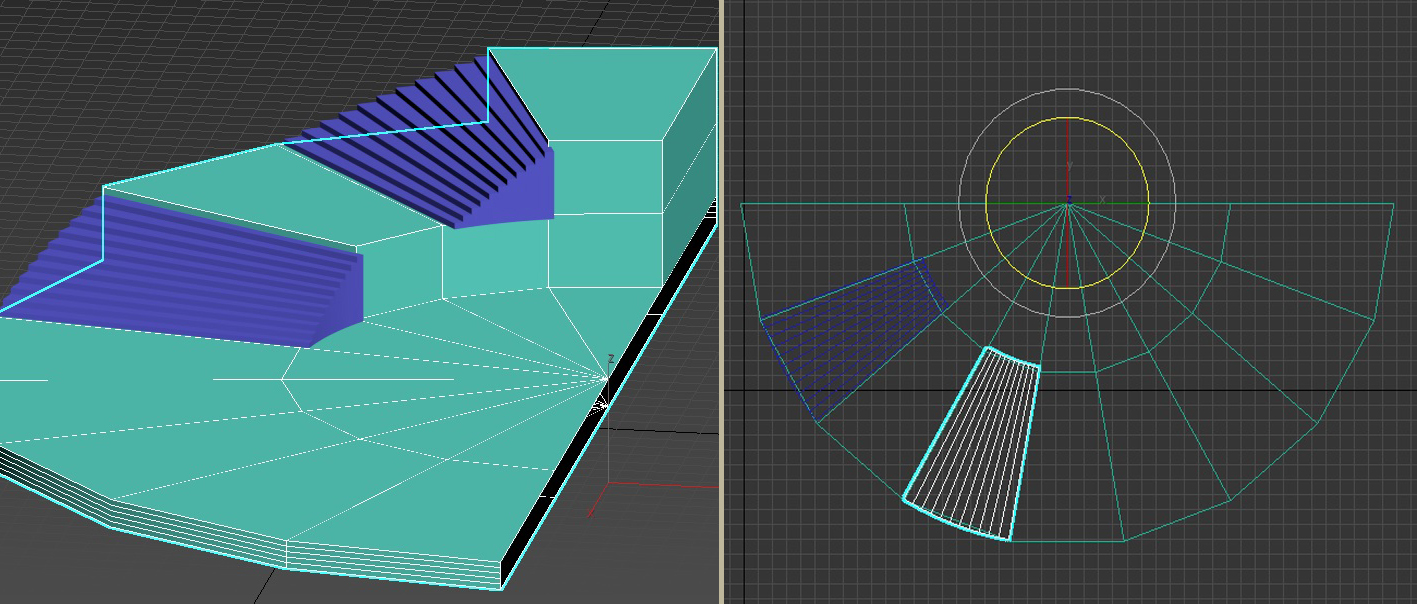
\includegraphics[width=0.95 \linewidth]{Abbildungen/3dsMax/Treppe_final}
	\caption{Treppenbau}
	\label{fig:Treppe}
\end{figure}

\begin{wrapfigure}{r}{0.3\textwidth}
	\begin{center}
		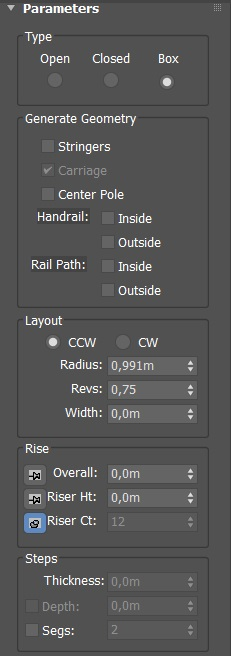
\includegraphics[width=0.25\textwidth]{Abbildungen/3dsMax/Treppe3}
	\end{center}
	\caption{Treppenparameter}
	\label{fig:Parameter}
\end{wrapfigure}

Um den erhöhten Innenring zu erreichen, musste eine Möglichkeit gefunden werden den Höhenunterschied auszugleichen. Treppen waren das Mittel der Wahl. Dazu wurde, wie in Abb. \ref{fig:Treppe} links zu sehen, die Außendecke mit dem\textit{Extrude} Befehl angepasst. Über die 3dsMax Objektauswahl können direkt Treppen als Grundobjekte erstellt werden. Da die Treppen in eine Rundung eingepasst werden sollten, wurden die \textit{SpiralStairs} gewählt. Abb. \ref{fig:Parameter} zeigt einen Ausschnitt der zu modifizierenden Parameter. Um einen geschlossenen Treppenkörper zu erhalten, wurde \textit(Box) gewählt. Der Radius der Treppe gleicht dem der Außendecke, um eine genaue Einpassung zu ermöglichen. Die Treppe wurde nun , wie in Abb. \ref{fig:Treppe} rechts gesehen, so verschoben, dass der Pivot Punkt der Treppe, dem der Außendecke entspricht. Um Sicherzustellen das später der First Person Controller die Treppen erklimmen kann, wurde darauf geachtet, dass Stufenhöhe und -tiefe Maßen entsprechen, welche auch in der Realität Anwendung finden. Dies ermöglichte der Parameter \textit{Riser Ht}, der zwischen 20cm - 30cm gewählt wurde. Auch im weiteren Modellierungsprozess wurden vermehrt Treppen eingesetzt, um die Begehung der Burg spannender zu gestalten.

\newpage
\subsection{Verfeinerung der Mauern}

\begin{figure}[h]
	\centering
	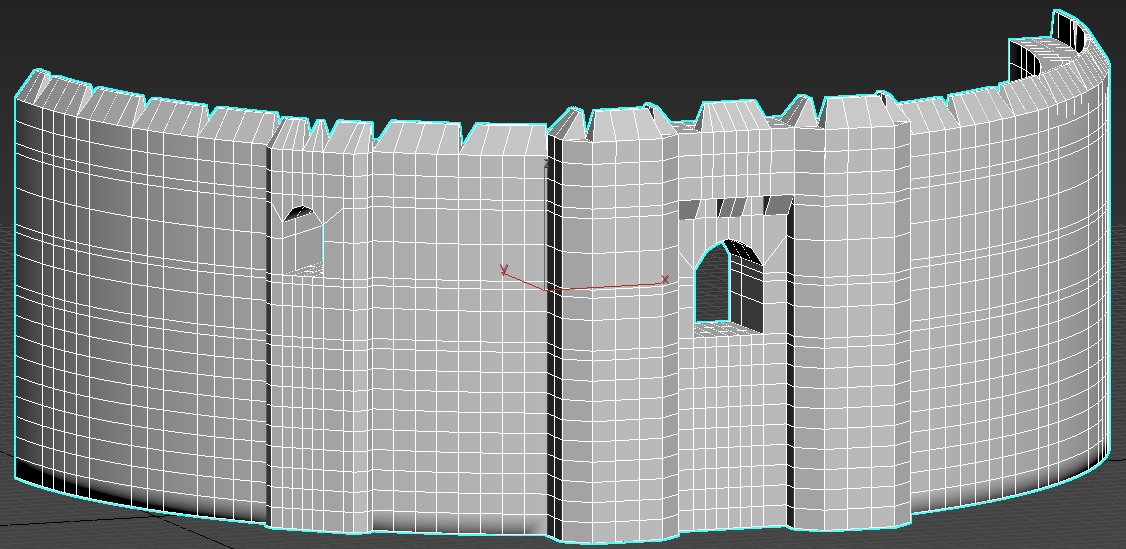
\includegraphics[width=0.95 \linewidth]{Abbildungen/3dsMax/Aussenring}
	\caption{Verfeinerung Außenring}
	\label{fig:Aussenring}
\end{figure}

Um den Außenring detaillierter zu gestalten, wurden hauptsächlich die Polygonwerkzeuge \textit{Extrude} und \textit{Bevel} genutzt. Durch paarweises auswählen und \textit{Bevel} wurden die Zinnen herausgearbeitet. Auch die obere Seite des Haupttores wurde mittels \textit{Extrude} detaillierter gestaltet. Um die Toröffnung herauszuarbeiten, wurden mithilfe des Kantenauswahlwerkzeugs \textit{Ring} alle horizontalen Kanten ausgewählt und mittels \textit{Connect} neue vertikale Kanten eingefügt. Durch gezieltes verschieben von Eckpunkten wurde die obere Rundung geforrmt. Der Durchgang wurde durch löschen der Polygone geschaffen und die daraus resultierenden offenen Fläche mithilfe des \textit{Bridge} Werkzeugs geschlossen. 

\begin{figure}[h]
	\centering
	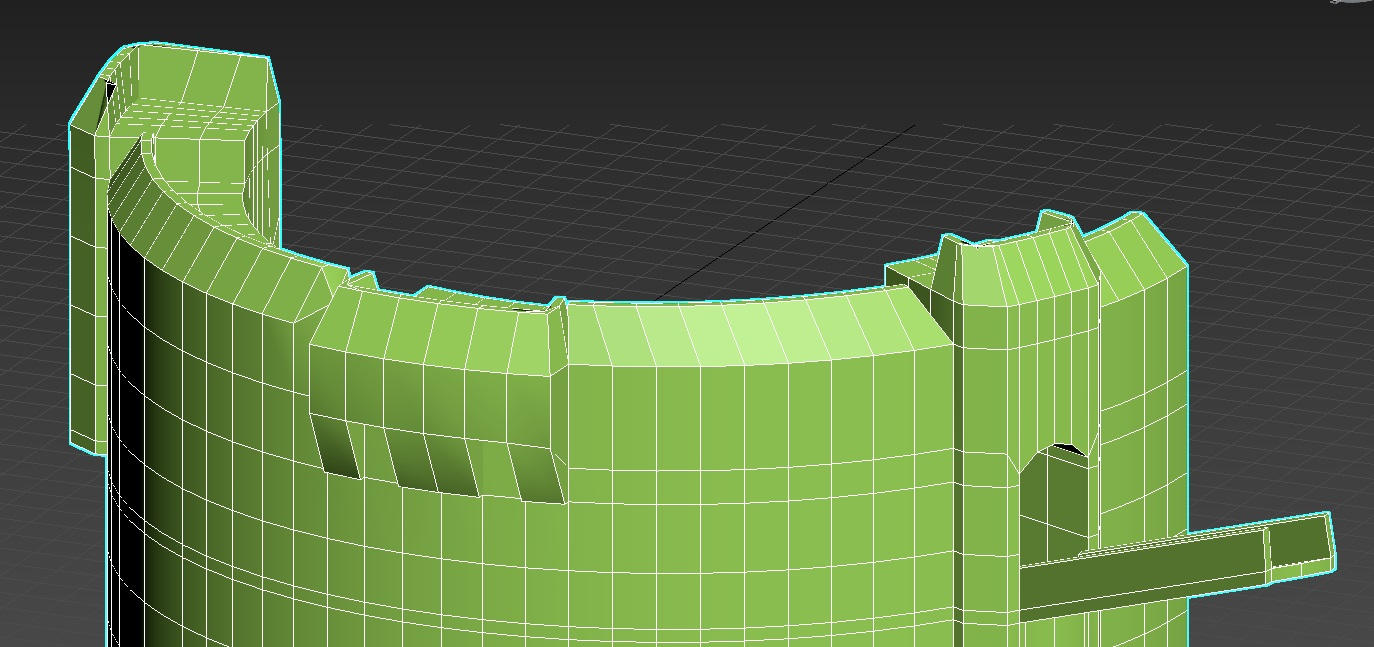
\includegraphics[width=0.95 \linewidth]{Abbildungen/3dsMax/Innenring}
	\caption{Verfeinerung Innenring}
	\label{fig:Innenring}
\end{figure}

Wie in Abb. \ref{fig:Innenring} zu sehen, wurde der Innenring ähnlich zum Außenring gestaltet, um einen einheitlichen Gesamteindruck zu erhalten. Die Zinnen sind aber ohne Schießscharten gehalten. Zum Abschluss wurde noch durch den \textit{Extrude} Befehl eine Brücke zum erreichen des Außenrings angefügt.

\begin{figure}[h]
	\centering
	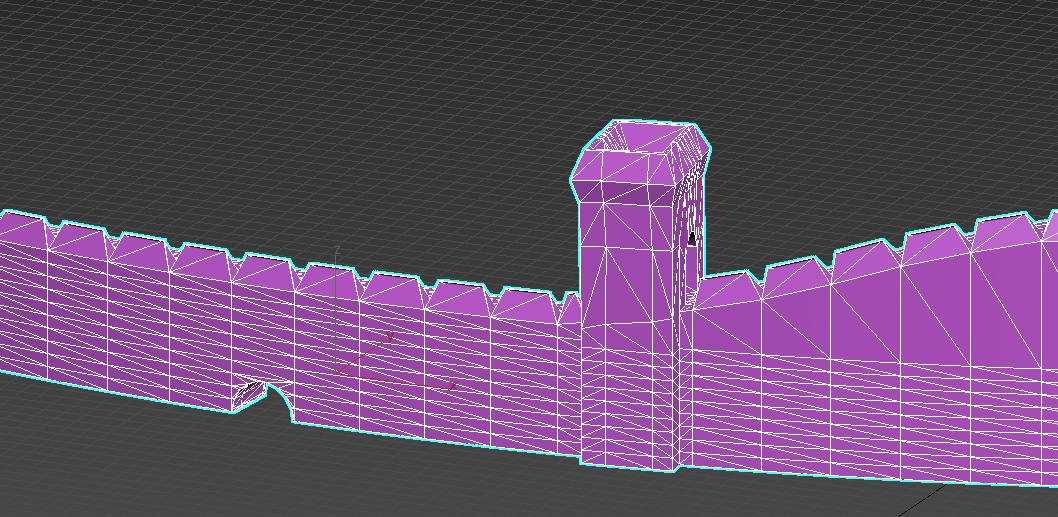
\includegraphics[width=0.95 \linewidth]{Abbildungen/3dsMax/Mauer}
	\caption{Verfeinerung Mauer}
	\label{fig:Mauer}
\end{figure}

Abb. \ref{fig:Mauer} zeigt die lange Verteidigungsmauer und den bereits erwähnten Flussdurchgang. Auch hier wurden Zinnen herausgearbeitet und des weiteren ein Wachturm mit Durchgang angefügt.
\newpage

\subsection{Haupthaus und Turm}

\begin{figure}[h]
	\centering
	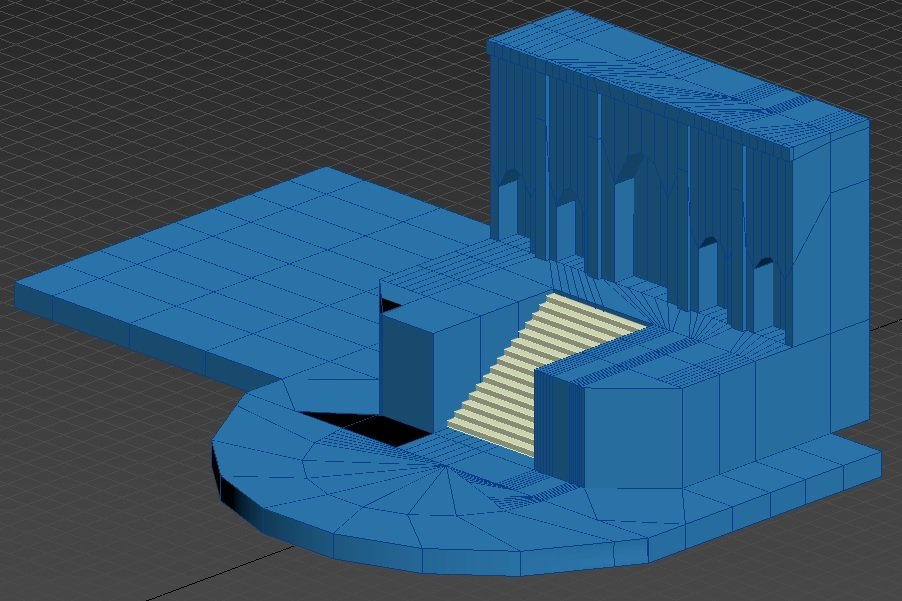
\includegraphics[width=0.95 \linewidth]{Abbildungen/3dsMax/Gebaeude}
	\caption{Haupthaus}
	\label{fig:Haupthaus}
\end{figure}

\begin{wrapfigure}[8]{r}{0.3\textwidth}
	\begin{center}
		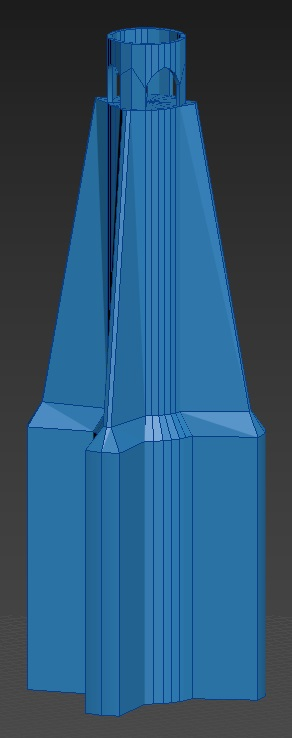
\includegraphics[width=0.22\textwidth]{Abbildungen/3dsMax/Turm}
	\end{center}
	\caption{Turm}
	\label{fig:Turm}
\end{wrapfigure}

Um Platz für das in Abb. \ref{fig:Haupthaus} zu sehende Haupthaus zu schaffen, wurde die halbrunde Innendecke mit mehrfachem Einsatz des \textit{Extrude} Befehls erweitert. Auch eine Plattform für den in Abb. \ref{fig:Turm} zu sehenden Turm wurde geschaffen. Der Turm besteht aus einem Zylinder, welcher durch das \textit{Extrude} und \textit{Bevel} Werkzeug in die gewünschte Form gebracht wurde. Ähnlich der Durchgänge, wurden Aussparungen am oberen Teil des Turmes angebracht.
\newpage

\subsection{Texturierung der Burg}

\begin{figure}[h]
	\centering
	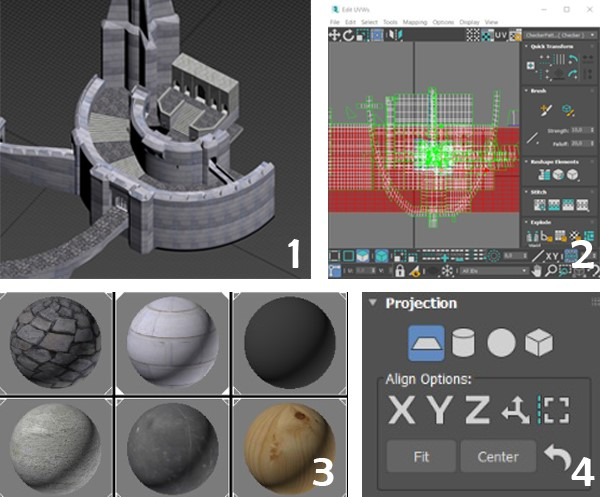
\includegraphics[width=0.95 \linewidth]{Abbildungen/3dsMax/Texturierung/Texturierung}
	\caption{Texturierung der Burg}
	\label{fig:textur}
\end{figure}

Zur Texturierung der Burg waren mehrere Schritte notwendig. Der erste Schritt umfasste das Aussuchen der Texturen. Im Internet wird eine Vielzahl an Texturen in Form von Bitmaps angeboten. Die ausgewählten Texturen wurden in den Materialeditor eingefügt (siehe Abb. \ref{fig:textur}.3)). Im nächsten Schritt wurden die Materialien den dazugehörigen Objekten zugeordnet. Durch eine Auswahl mit dem Polygonwerkzeug konnten auch mehrere Texturen auf ein Objekt angewendet werden. Nach der Zuordnung der Materialien fiel auf, dass die Texturen verzerrt waren. Dies liegt daran, dass 3dsMax komplexe Objekte nicht automatisch in Ihre sogenannte \textit{UVW Map} zerlegen kann. Diese Zerlegung musste per Hand erfolgen. Dazu wendet man auf das Objekt den Modifikator \textit{Unwrap UVW} an. Nun kann man über den \textit{UV Editor}(siehe Abb. \ref{fig:textur}).2) die UV Map per Hand bearbeiten, skalieren und drehen. Abb. \ref{fig:textur}.1 zeigt die fertig texturierte Burg.
\newpage

\subsection{Animationen in 3dsMax}
\subsubsection{Katapult}

\begin{figure}[h]
	\centering
	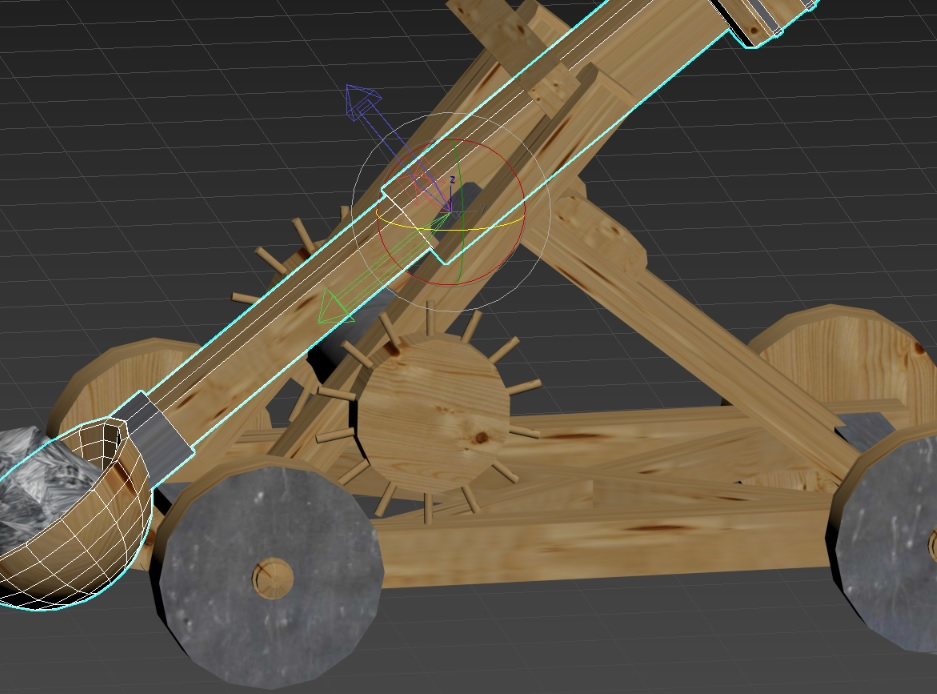
\includegraphics[width=0.95 \linewidth]{Abbildungen/3dsMax/catapult}
	\caption{Katapult}
	\label{fig:catapult}
\end{figure}

\begin{wrapfigure}[14]{r}{0.3\textwidth}
	\begin{center}
		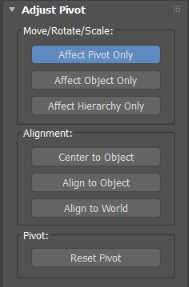
\includegraphics[width=0.3\textwidth]{Abbildungen/3dsMax/pivot}
	\end{center}
	\caption{Pivot Einstellung}
	\label{fig:Pivot}
\end{wrapfigure}

Im Unity Assetstore findet sich das in Abb. \ref{fig:catapult} zu sehende Katapult, welches aus zwei Teilen besteht, dem Fahrwerk und dem Katapultarm. Der Katapultarm sollte animiert werden um einen Stein abfeuern zu können. An erster Stelle musste der Pivotpunkt des Armes verschoben werden, um eine Drehung um die richtige Position zu ermöglichen. Dazu wechselt man in die Hierachie Einstellung und wählt \textit{Affect Pivot Only} (siehe Abb. \ref{fig:Pivot}). Nun kann man den Pivot Punkt beliebig verschieben. Istr die richtige Position gefunden, aktiviert man den \textit{Auto-Key} Modus, um Keyframes für die Animation zu erstellen. Der erste Keyframe wird automatisch am Anfang gesetzt. Nun dreht man den Katapultarm zu seiner Endposition, wählt in der Zeitleiste einen späteren Zeitpunkt und ein neuer Keyframe wird gesetzt. Damit ist die Animation abgeschlossen. Identisch wurde mit dem zu feuerendem Stein verfahren, mit der Ausnahme, dass die Animation noch mit der Flugkurve des Steines erweitert wurde. Diese führt durch das zu treffende Objekt (Mauer) und endet dahinter (auf dem Boden).

\subsubsection{Mauer}
\begin{figure}[h]
	\centering
	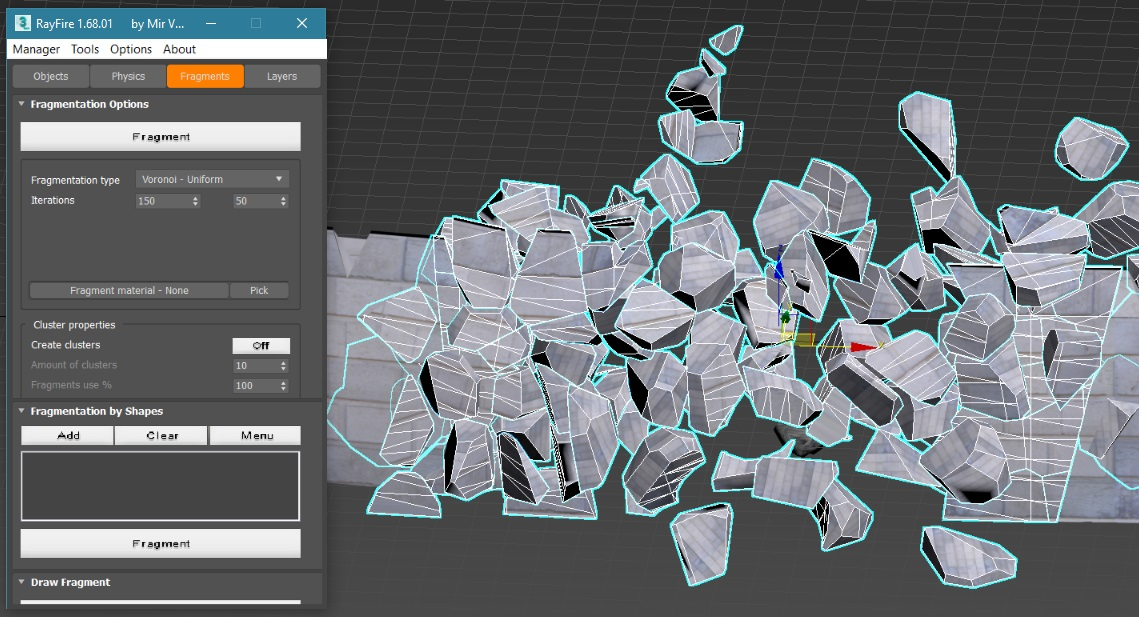
\includegraphics[width=0.95 \linewidth]{Abbildungen/3dsMax/rayfire}
	\caption{Mauerexplosion}
	\label{fig:rayfire}
\end{figure}
Um die Mauer bei Steineinschlag zerspringen zu lassen, wurde die Demoversion des 3dsMax Plugins \textit{Rayfire} verwendet. Um dieses Plugin nutzen zu können, wählt man es aus der Objektliste aus. Darauffolgend öffnet sich der in Abb. \ref{fig:rayfire} zu sehende Dialog. Durch sogenanntes fragmentieren wird die Mauer automatisch in viele unförmige Teile zerlegt. Diese dienen später als Splitter der Explosion. Nach dem einstellen des Animationsbeginn und -ende, kann man nun den beteiligten Objekten ihre Rollen zuweisen. Die Mauerobjekte sind sogenannte \textit(Sleeping Objects). Das bedeutet sie bleiben an Ort und Stelle bis ein sogenanntes \textit{Kinematic Object} auf sie einwirkt. Diese Rolle übernimmt der Stein, welcher im Laufe seiner Animation durch die Mauer fliegt. Wurden nun alle Einstellungen getroffen, kann man sich über den \textit{Preview} Button das Resultat ansehen. Ist man mit diesem zufrieden, werden die Keyframes der Animation mit dem \textit{Bake} Befehl generiert. Nach diesem Befehl ist ein bearbeiten der Animation nicht mehr möglich.
 